\documentclass[10pt]{article}\usepackage[]{graphicx}\usepackage[]{color}
%% maxwidth is the original width if it is less than linewidth
%% otherwise use linewidth (to make sure the graphics do not exceed the margin)
\makeatletter
\def\maxwidth{ %
  \ifdim\Gin@nat@width>\linewidth
    \linewidth
  \else
    \Gin@nat@width
  \fi
}
\makeatother

\definecolor{fgcolor}{rgb}{0.345, 0.345, 0.345}
\newcommand{\hlnum}[1]{\textcolor[rgb]{0.686,0.059,0.569}{#1}}%
\newcommand{\hlstr}[1]{\textcolor[rgb]{0.192,0.494,0.8}{#1}}%
\newcommand{\hlcom}[1]{\textcolor[rgb]{0.678,0.584,0.686}{\textit{#1}}}%
\newcommand{\hlopt}[1]{\textcolor[rgb]{0,0,0}{#1}}%
\newcommand{\hlstd}[1]{\textcolor[rgb]{0.345,0.345,0.345}{#1}}%
\newcommand{\hlkwa}[1]{\textcolor[rgb]{0.161,0.373,0.58}{\textbf{#1}}}%
\newcommand{\hlkwb}[1]{\textcolor[rgb]{0.69,0.353,0.396}{#1}}%
\newcommand{\hlkwc}[1]{\textcolor[rgb]{0.333,0.667,0.333}{#1}}%
\newcommand{\hlkwd}[1]{\textcolor[rgb]{0.737,0.353,0.396}{\textbf{#1}}}%
\let\hlipl\hlkwb

\usepackage{framed}
\makeatletter
\newenvironment{kframe}{%
 \def\at@end@of@kframe{}%
 \ifinner\ifhmode%
  \def\at@end@of@kframe{\end{minipage}}%
  \begin{minipage}{\columnwidth}%
 \fi\fi%
 \def\FrameCommand##1{\hskip\@totalleftmargin \hskip-\fboxsep
 \colorbox{shadecolor}{##1}\hskip-\fboxsep
     % There is no \\@totalrightmargin, so:
     \hskip-\linewidth \hskip-\@totalleftmargin \hskip\columnwidth}%
 \MakeFramed {\advance\hsize-\width
   \@totalleftmargin\z@ \linewidth\hsize
   \@setminipage}}%
 {\par\unskip\endMakeFramed%
 \at@end@of@kframe}
\makeatother

\definecolor{shadecolor}{rgb}{.97, .97, .97}
\definecolor{messagecolor}{rgb}{0, 0, 0}
\definecolor{warningcolor}{rgb}{1, 0, 1}
\definecolor{errorcolor}{rgb}{1, 0, 0}
\newenvironment{knitrout}{}{} % an empty environment to be redefined in TeX

\usepackage{alltt}

\usepackage{amsmath,amssymb,amsthm}
\usepackage{fancyhdr,url,hyperref}
\usepackage{graphicx,xspace}
\usepackage{subfigure}
\usepackage{tikz}
\usetikzlibrary{arrows,decorations.pathmorphing,backgrounds,positioning,fit,through}

\oddsidemargin 0in  %0.5in
\topmargin     0in
\leftmargin    0in
\rightmargin   0in
\textheight    9in
\textwidth     6in %6in
%\headheight    0in
%\headsep       0in
%\footskip      0.5in

\newtheorem{thm}{Theorem}
\newtheorem{cor}[thm]{Corollary}
\newtheorem{obs}{Observation}
\newtheorem{lemma}{Lemma}
\newtheorem{claim}{Claim}
\newtheorem{definition}{Definition}
\newtheorem{question}{Question}
\newtheorem{answer}{Answer}
\newtheorem{problem}{Problem}
\newtheorem{solution}{Solution}
\newtheorem{conjecture}{Conjecture}

\pagestyle{fancy}

\lhead{\textsc{Prof. McNamara}}
\chead{\textsc{SDS/MTH 220: Lecture notes}}
\lfoot{}
\cfoot{}
%\cfoot{\thepage}
\rfoot{}
\renewcommand{\headrulewidth}{0.2pt}
\renewcommand{\footrulewidth}{0.0pt}

\newcommand{\ans}{\vspace{0.25in}}
\newcommand{\R}{{\sf R}\xspace}
\newcommand{\cmd}[1]{\texttt{#1}}
\newcommand{\Ex}{\mathbb{E}}

\rhead{\textsc{November 2017, 2017}}
\IfFileExists{upquote.sty}{\usepackage{upquote}}{}
\begin{document}

\paragraph{Agenda}
\begin{enumerate}
  \itemsep0em
  \item Inference for Regression
  \item Conditions for Regression
\end{enumerate}

\paragraph{Regression}

Consider the following data about US states. We fit a simple linear regression line for the poverty rate in each state as a function of the high school graduation rate. 

\begin{knitrout}\footnotesize
\definecolor{shadecolor}{rgb}{0.969, 0.969, 0.969}\color{fgcolor}\begin{kframe}
\begin{alltt}
\hlkwd{require}\hlstd{(mosaic)}
\hlstd{poverty} \hlkwb{<-} \hlkwd{read.csv}\hlstd{(}\hlstr{"http://math.smith.edu/~bbaumer/mth241/poverty.txt"}\hlstd{,} \hlkwc{sep} \hlstd{=} \hlstr{"\textbackslash{}t"}\hlstd{)}
\hlstd{mod} \hlkwb{<-} \hlkwd{lm}\hlstd{(Poverty} \hlopt{~} \hlstd{Graduates,} \hlkwc{data} \hlstd{= poverty)}
\hlkwd{coef}\hlstd{(mod)}
\end{alltt}
\begin{verbatim}
## (Intercept)   Graduates 
##  64.7809658  -0.6212167
\end{verbatim}
\end{kframe}
\end{knitrout}

\begin{enumerate}
  \item Write a sentence providing an interpretation of the coefficient for $Graduates$ in the context of the problem. 
  \vspace{0.5in}
\end{enumerate}

\paragraph{Inference for Regression}

We can use our understanding of the $t$-distribution to make \emph{inferences} about the true (unknown) value of regression coefficients. In particular, we can test the hypothesis that $\beta_1 = 0$ and find a confidence interval for $\beta_1$. 

\begin{knitrout}\footnotesize
\definecolor{shadecolor}{rgb}{0.969, 0.969, 0.969}\color{fgcolor}\begin{kframe}
\begin{alltt}
\hlkwd{summary}\hlstd{(mod)}
\end{alltt}
\begin{verbatim}
## 
## Call:
## lm(formula = Poverty ~ Graduates, data = poverty)
## 
## Residuals:
##     Min      1Q  Median      3Q     Max 
## -4.1624 -1.2593 -0.2184  0.9611  5.4437 
## 
## Coefficients:
##             Estimate Std. Error t value Pr(>|t|)    
## (Intercept) 64.78097    6.80260   9.523 9.94e-13 ***
## Graduates   -0.62122    0.07902  -7.862 3.11e-10 ***
## ---
## Signif. codes:  0 '***' 0.001 '**' 0.01 '*' 0.05 '.' 0.1 ' ' 1
## 
## Residual standard error: 2.082 on 49 degrees of freedom
## Multiple R-squared:  0.5578,	Adjusted R-squared:  0.5488 
## F-statistic: 61.81 on 1 and 49 DF,  p-value: 3.109e-10
\end{verbatim}
\end{kframe}
\end{knitrout}

\begin{enumerate}
  \itemsep0.5in
  \item Find a 95\% confidence interval and $p$-value for the slope coefficient.
  \item What do you conclude about the association between poverty rates and high school graduation rates among US states? 
  \vspace{0.5in}
\end{enumerate}


\paragraph{Example: Gestation}

The \texttt{Gestation} data set contains birth weight, date, and gestational period collected as part of the Child Health and Development Studies in 1961 and 1962. Information about the baby's parents---age, education, height, weight, and whether the mother smoked is also recorded.

\begin{enumerate}
  \itemsep1in
  \item Fit a linear regression model for birthweight ($wt$) as a function of the mother's age ($age$).
  \item Use the {\tt summary} command to find a 95\% confidence interval and $p$-value for the slope coefficient
  \item What do you conclude about the association between a mother's age and her baby's birthweight?
  \vspace{0.5in}
\end{enumerate}


\paragraph{Conditions for Regression}

The inferences we made above were predicted upon our assumption that the slope coefficient followed a $t$-distribution. Recall also that when we fit the regression model
$$
  Y = \beta_0 + \beta_1 \cdot X + \epsilon \, ,
$$
we assumed that $\epsilon \sim N(0, \sigma)$, for some constant $\sigma$. Our inferences will only be valid if the following assumptions are reasonable: 

\begin{itemize}
  \itemsep0in
  \item \textbf{L}inearity:
  \item \textbf{I}ndependence:
  \item \textbf{N}ormality of Residuals:
  \item \textbf{E}qual Variance of Residuals:
\end{itemize}
\clearpage
These conditions are usually verified using diagnostic plots. 

\begin{knitrout}
\definecolor{shadecolor}{rgb}{0.969, 0.969, 0.969}\color{fgcolor}\begin{kframe}
\begin{alltt}
\hlkwd{plot}\hlstd{(mod,} \hlkwc{which}\hlstd{=}\hlkwd{c}\hlstd{(}\hlnum{1}\hlstd{,}\hlnum{2}\hlstd{))}
\end{alltt}
\end{kframe}
\end{knitrout}

\begin{knitrout}
\definecolor{shadecolor}{rgb}{0.969, 0.969, 0.969}\color{fgcolor}\begin{kframe}
\begin{verbatim}
## NULL
## NULL
\end{verbatim}
\end{kframe}
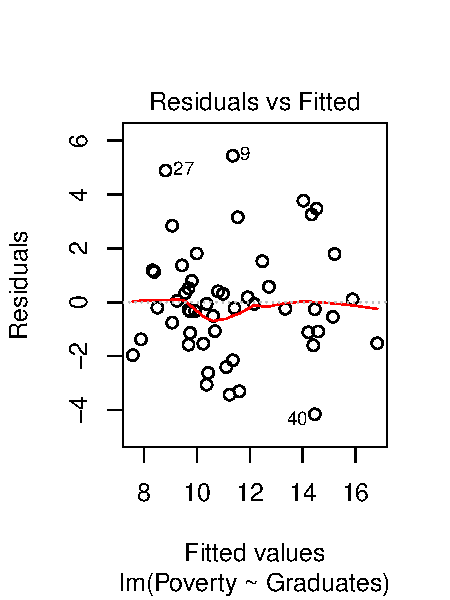
\includegraphics[width=\maxwidth]{figure/unnamed-chunk-4-1} 
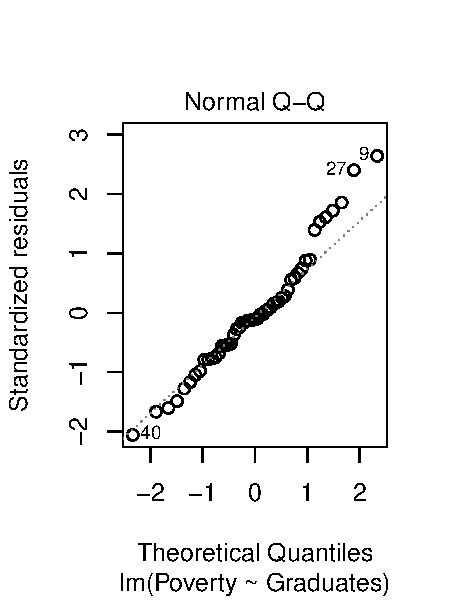
\includegraphics[width=\maxwidth]{figure/unnamed-chunk-4-2} 

\end{knitrout}

\clearpage
\paragraph{Practice Problems}
\begin{enumerate}
  \item Verify the conditions for the US states model above.
  \item Verify the conditions for the Gestation model above. 
  \item (EOCE 5.17) The Association of Turkish Travel Agencies reports the number of foreign tourists visiting Turkey and tourist spending by year. The scatterplot below shows the relationship between these two variables along with the least squares fit.
  
\begin{knitrout}
\definecolor{shadecolor}{rgb}{0.969, 0.969, 0.969}\color{fgcolor}
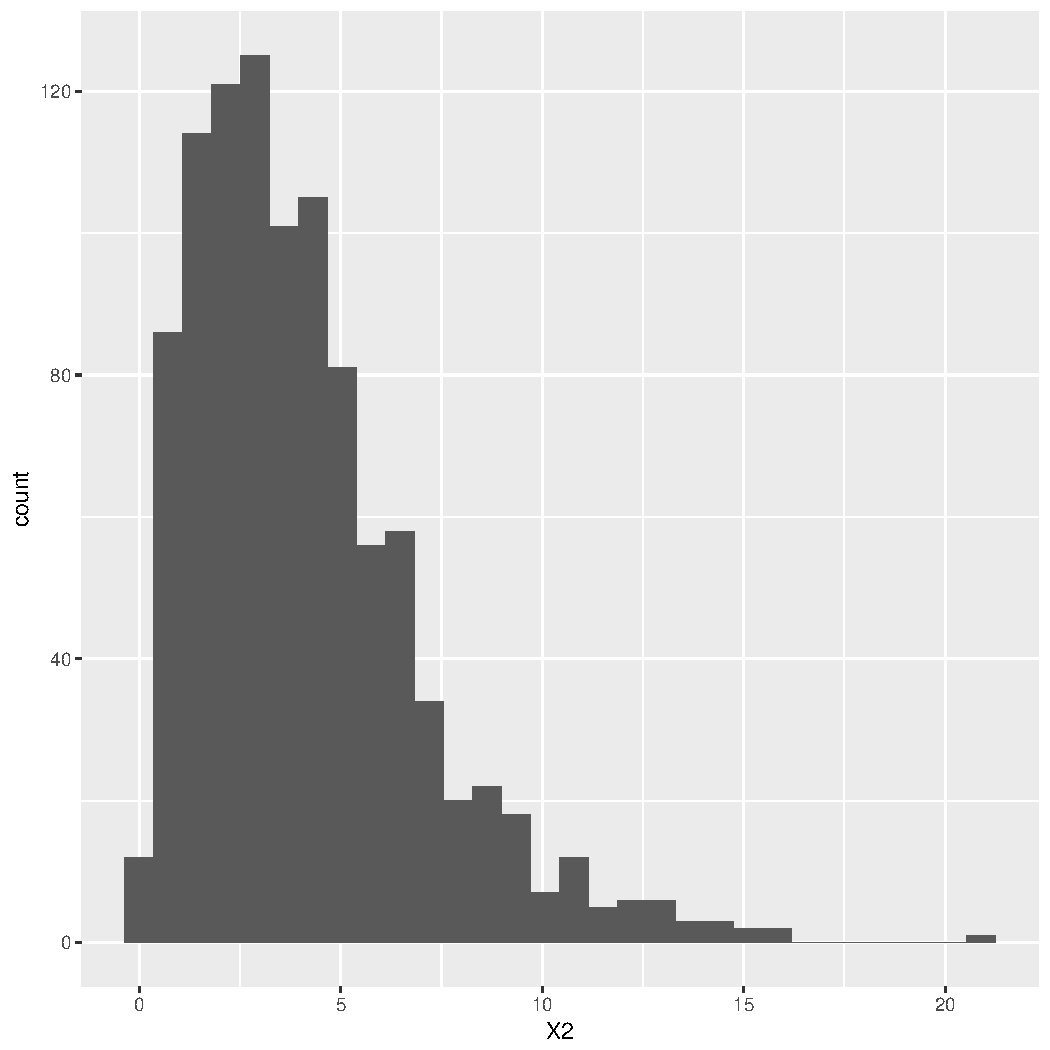
\includegraphics[width=\maxwidth]{figure/unnamed-chunk-5-1} 

\end{knitrout}

  \begin{enumerate}
    \itemsep0.5in
    \item Describe the relationship between number of tourists and spending.
    \item What are the explanatory and response variables?
    \item Why might we want to fit a regression line to these data?
    \item Do the data meet the conditions required for fitting a least squares line? In addition to the scatterplot, use the residual plot and histogram to answer this question.
  \end{enumerate}

\end{enumerate}

% \newpage
% 
% \paragraph{Inference for Regression}
% 
% Just as we are able to make inferences about population means, we can make inferences about parameters in a regression model.
% 
% \begin{itemize}
%   \item Note that the confidence intervals we discussed above are of the form:
% $$
%   \text{estimate} \pm \text{multiplier} \cdot \text{standard error}
% $$
% In the same manner, when we fit a regression model of the form
% $$
%   Y = \beta_0 + \beta_1 \cdot X + \epsilon \, ,
% $$
% we find $t$-confidence intervals for each coefficient of the form:
% $$
%   \hat{\beta_i} \pm \text{multiplier} \cdot \text{standard error}_{\beta_i}
% $$
%   \item We are particularly interested in testing the hypothesis that $\beta_1 = 0$. [Why?]
%   \item The test statistic is: $t_{\beta_1} = \frac{\hat{\beta_1} - 0}{SE_{\beta_1}}$.
%   \item The degrees of freedom is $(n-1) - \text{\# of predictors}$.
% \end{itemize}
% 
% \paragraph{Warmup}
% 
% Poverty and graduation rate
% 
% <<>>=
% summary(mod)
% confint(mod)
% @
% 
% \paragraph{Solution to Gestation}
% 
% birthweight of babies
% 
% <<fig.show='hide'>>=
% require(mosaicData)
% fm <- lm(wt ~ age, data = Gestation)
% summary(fm)
% confint(fm)
% plot(fm)
% @


\end{document}
